The thermal model has been built as described in Section \ref{subsec:thermaltool} according to the method explained by Smith et al. \cite{Smith2011}. Before the model can be used for the design it has to undergo the verification and validation process. In the first part the verification is done by comparing the analytical and numerical solutions of a copper block. In the second part two papers by Del Corso et al. are used to validate the developed model with experimental data \cite{Corso2009,Corso2011}. The last part will explain the differences that were found in the verification and validation.

\subsubsection{Verification of the model using a solid copper block}
For the verification of the thermal model the analytical solution (Equation \eqref{eq:thermver}) provided by both Smith and Holman is used \cite{Smith2011,Holman2002}. Here $\gls{sym:T}_1$ is the wall temperature at $\gls{sym:t}=0$ and $\gls{sym:T}_2$ the temperature at a certain $\gls{sym:t} \left[s\right]$ and $\gls{sym:x}$.
\begin{equation}
\gls{sym:T}_2-\gls{sym:T}_1 = \frac{2\dot{q}\sqrt{\gls{sym:alphat}\gls{sym:t}/\pi}}{\gls{sym:k}\gls{sym:A}}\exp\left(\frac{-\gls{sym:x}^2}{4\gls{sym:alphat}\gls{sym:t}}\right)-\frac{\dot{q}\gls{sym:x}}{\gls{sym:k}\gls{sym:A}}\left(1-erf\frac{\gls{sym:x}}{2\sqrt{\gls{sym:alphat}\gls{sym:t}}}\right)
\label{eq:thermver}
\end{equation}
Figure \ref{fig:valcop} shows a semi-infinite $0.5 \left[m\right]$ thick copper block subjected to a constant heat flux of $30 \left[W\cdot cm^{-2}\right]$. The block initially has a uniform temperature of $20 \left[^{\circ}C\right]$. The error at the surface ($x = 0.00 \left[m\right]$), in the middle ($x = 0.25 \left[m\right]$) and at the back ($x = 0.50 \left[m\right]$) between the analytical and numerical solution are $1.55\%$, $4.32\%$ and $15.92\%$ respectively.

\begin{figure}[H]
	\centering
	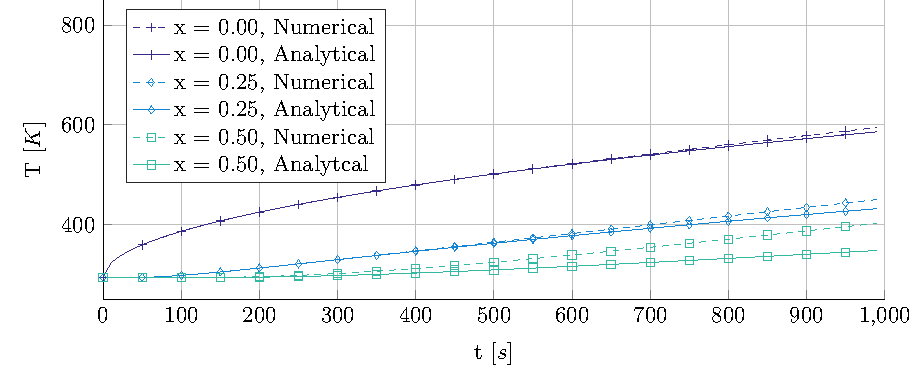
\includegraphics{Figure/Thermal/valcop.pdf}
	\caption[Comparison of analytical and numerical solution using a copper block]{Comparison of analytical and numerical solution by applying a constant heat flux for $1000 \left[s\right]$ on a copper block with a $0.5 \left[m\right]$ thickness.}
	\label{fig:valcop}
\end{figure}

\subsubsection{Validation against experimental data}
As mentioned earlier two papers by Del Corso et al. provide the experimental data \cite{Corso2009,Corso2011}. The four lay-ups shown in Figure \ref{fig:vallayup} have been tested to validate the thermal model. Note that the references do not provide the experimental data for lay-up 1, but give the result of the thermal model they have used. For lay-up 2 and 3 data from both \gls{nasa}'s model and experiments have been provided. 


\begin{figure}[h]
	\centering
	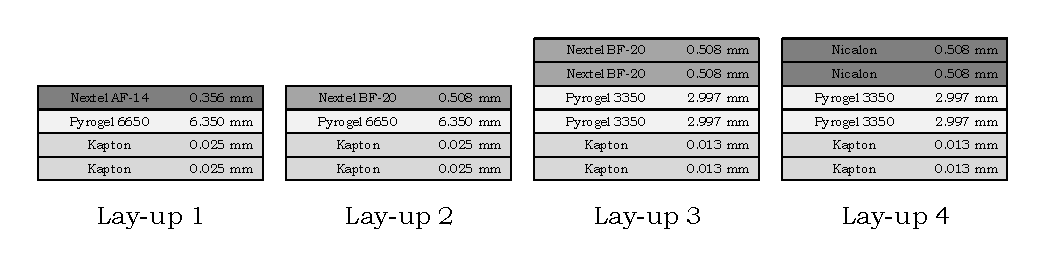
\includegraphics[width=\textwidth]{Figure/Thermal/vallayup.pdf}
	\caption{The four lay-ups used to test the thermal model against experimental data}
	\label{fig:vallayup}
\end{figure}

All lay-ups have been compared and validated. Before the model is validated all the contact resistances had to be adjusted such that they match the experimental data as was already mentioned in Section \ref{subsec:thermaltool}. The reason for this is that it is not possible to determine this value analytically. Lay-up 2 is used to serve as an example of this validation and has been subjected to a heat flux of $6.2 \left[W\cdot cm^{-2}\right]$ for $90 \left[s\right]$. Between every layer a thermocouple was placed during the experiment. With four layers that means that there were three thermocouples. Figure \ref{fig:plotvallay2} shows the result of this validation. It is clear that the model works very well during the application of the heat flux in the first $90 \left[s\right]$. The average error for thermocouples TC1, TC2 and TC3 are 3.9\%, 3.0\% and 4.8\% respectively. However, during the cooling down of the lay-up the error rapidly increases to 60.1\%, 66.0\% and 68.9\%.

\begin{figure}[H]
	\centering
	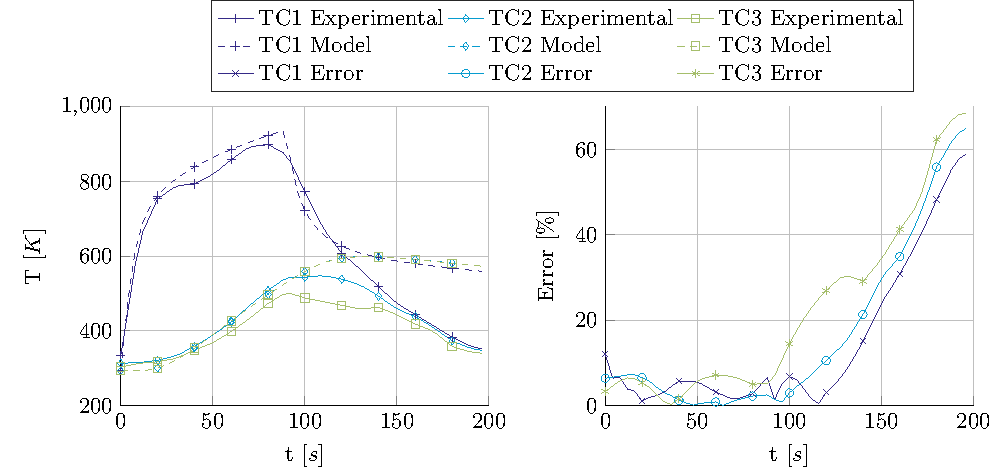
\includegraphics[width=\textwidth]{Figure/Thermal/plotvallay2.pdf}
	\caption{Thermal model compared to experimental data at three locations}
	\label{fig:plotvallay2}
\end{figure}

Table \ref{tab:valerrorthermo} shows the result of all the lay-ups. The thermal model has been compared to \gls{nasa}'s model, the experimental data where possible. For reference NASA's model has been compared to the experimental data to show the performance of the developed thermal model. Note that the maximum error is the average of the maximum errors of the thermocouples. Also for every lay-up the contact resistance must be tweaked in order to match the experimental data. The number used in tweaking is characteristic for the two layers it separates. The table shows that the thermal model is accurate to about 15 to 20\%. The fourth layer with Nicalon\textsuperscript{TM} has a high average error, this is due to the relatively high errors in the Pyrogel\textsuperscript{\textregistered} and kapton layers. The temperature in the Nicalon\textsuperscript{TM} layer is correctly modelled with the same 15 to 20\% accuracy. \gls{nasa}'s model performs better with an accuracy of about 10 to 15\%. Not visible in the table, but visible in Figure \ref{fig:plotvallay2} is that larger errors in the cooling down phases are overestimates of the temperatures.

\begin{table}[h]
	\centering
	\caption{Comparison of thermal model, \acrshort{nasa}'s model and experimental data}
	\begin{tabular}{|p{5.6cm}|rrrr|}
		\hline
		\textbf{} & \textbf{Lay-up 1} & \textbf{Lay-up 2} & \textbf{Lay-up 3} & \textbf{Lay-up 4} \\ \hline \hline
		\multicolumn{5}{|l|}{\textbf{Thermal model vs. experimental data}}			\\ \hline	
		Avg. error											&        - & 18.28\% & 16.45\% & 30.87\% \\
		Max. error											&        - & 65.03\% & 70.90\% & 56.25\% \\
		Avg. error during heat flux							&        - &  3.91\% & 17.75\% & 31.37\% \\
		Avg. error during cooling down						&        - & 30.05\% &  8.67\% & 27.52\% \\ \hline
		\multicolumn{5}{|l|}{\textbf{Thermal model vs. \gls{nasa}'s model}}			\\ \hline		
		Avg. error											&   6.72\% & 10.88\% & 17.85\% &        - \\
		Max. error											&  22.54\% & 22.42\% & 55.56\% &        - \\
		Avg. error during heat flux							&   7.26\% & 10.48\% & 18.19\% &        - \\
		Avg. error during cooling down						&   6.62\% & 11.20\% & 15.84\% &        - \\ \hline
		\multicolumn{5}{|l|}{\textbf{\gls{nasa}'s model vs. experimental data}}			\\ \hline		
		Avg. error											&        - & 13.79\% & 10.69\% &        - \\
		Max. error											&        - & 43.37\% & 34.22\% &        - \\
		Avg. error during heat flux							&        - &  8.43\% & 10.28\% &        - \\
		Avg. error during cooling down						&        - & 18.18\% & 13.15\% &        - \\ \hline
	\end{tabular}
	\label{tab:valerrorthermo}
\end{table}


\subsubsection{Conclusions after the verification and validation procedure}
The verification showed that the numerical solution starts to diverge as the error increases with time and depth. It is expected that this is a result of rounding errors that get multiplied every time step in the discretisation scheme. The reason for this is that refining the mesh produces the same errors. There are two reasons why this is not a significant problem for the design problem. The first is that the \gls{tps} shall be a hundred times thinner. The second is that the length of the aerocapture and entry phases are approximately $800 \left[s\right]$, which is within the verified duration. 
 
The validation shows that the thermal model, with an accuracy of 15 to 20\%, performs slightly worse than \gls{nasa}'s model with an accuracy of 10 to 15\%. It is assumed that errors under 10\% should be completely acceptable for a low fidelity model. Larger error should be contributed to the difficulties in contact resistance modelling. When increasing the amount of layers it is increasingly difficult to predict the contact resistance, something Del Corso also experienced in \gls{nasa}'s model \cite{Corso2009}. This especially gets worse when there is no heat applied and the lay-up converges to an equilibrium state. For the purpose of the design of the lay-up for an inflatable heat shield this is not a problem, as the heat shield has enough time to cool down in the parking orbit after the aerocapture before it starts its final entry. For these reasons the thermal model is considered validated and safe to use for design while keeping its accuracy in mind.